\chapter{Conclusions and future work}\label{chp:chp7}

\begin{flushright}
  {\em ``My real love has always been the sleep that rescued me by allowing me to dream.''}\\

\ \

\normalsize
{Luigi Pirandello}  
\end{flushright}


\noindent{In this thesis, I have explored the properties of tens of millions of galaxies that have been observed by the Dark Energy Survey to study gravitational wave sources and dark matter in galaxy clusters. All of the analyses performed are easily transferrable to larger future datasets, which will include the final DES data and a larger number of LIGO events in the near future, and LSST data in the longer term.}

In Chapter 2, I have presented the methods used to derive redshifts, stellar masses, and other properties of galaxies from photometric surveys. In particular, I have shown how a Bayesian Model Averaging method has been developed and applied in my work for galaxies in clusters studies. This method naturally takes into account the uncertainties due to the model selection, and working with a code that I developed has provided me with the flexibility needed to perform the varied analyses presented in the following chapters. The outputs of these methods have been used for two different science cases, both of which have important implications for cosmology: an understanding of galaxies and their evolution is a fundamental step towards unlocking the dark sector of the Universe.

\section{Gravitational waves}

The discovery of the first gravitational wave signal from a binary neutron star coalescence, GW170817, and its associated electromagnetic counterpart has been a milestone in the history of astronomy. The identification of the galaxy that hosted this event (and a careful characterisation of its redshift) has allowed new constraints to be placed on the Hubble constant, although currently not as stringent as those from more traditional methods. 

\subsection{Conclusions from this thesis}
In this thesis, I have shown that an analysis of the host galaxy can also provide useful information on the formation mechanisms and evolution of binary neutron stars, which are still poorly understood. By applying these concepts to the host galaxy of GW170817, NGC 4993, I have described the extensive morphological and spectral analyses performed. The results show that NGC 4993 is an early--type galaxy, with $i$-band S\'ersic index $n=4.0$ and low asymmetry ($A=0.04\pm 0.01$), which is unusual for sGRB hosts. However, shell structures, dust lanes and photometric properties are consisted with a disturbed galaxy that has likely undergone a recent galaxy merger. Neither spatially--resolved broadband SED, spectral fitting nor pixel color--magnitude analyses show evidence for recent star formation. The best--fit SFH has been used to estimate the BNS merger rate in this type of galaxy when a pure star formation scenario is assumed for BNS formation: $R_{NSM}^{gal}= 5.7^{+0.57}_{-3.3} \times 10^{-6} {\rm yr}^{-1}$. This type of calculation has been extended to all observable early type galaxies in the volume which is observable by LIGO, obtaining $0.038^{+0.004}_{-0.022}$ events in total for the LIGO observing seasons O1 and O2. In the pure SF scenario, most of the contribution to the expected number of observable events comes from late--type, star forming galaxies, summing up to $\sim 0.5$ events from all galaxy types. These numbers, together with the observation of GW170817 in NGC 4993, suggest that pure star formation may not be the only formation mechanism of BNSs. I have suggested that dynamical interactions may have affected the formation or evolution of the system. If such interactions arose during the galaxy merger, the subsequent time elapsed can constrain the delay time of the BNS coalescence. By using velocity dispersion estimates and the position of the shells, I find that the galaxy merger occurred $t_{\rm mer}\lesssim 200~{\rm Myr}$ prior to the BNS coalescence. 

Other authours have followed our line of thought and reached similar conclusions. \citet{Belczynski} probe different formation mechanisms of double compact objects and find that these are unlikely to happen in this type of galaxy, suggesting that the observation of this event in NGC 4993 is either statistically unlickely, or that formation mechanisms need to be revised. \citet{ebrova} have described in more analytical detail the shells of NGC 4993 from HST data, finding that the galaxy merger happened around $\sim 400$ Myr ago. If this is a more accurate estimate of the time since the galaxy merger than our value, then it should be used as an estimate of time delay from a dynamically driven formation model. However, this does not affect our conclusions.

In Chapter 3, I have also presented the role of galaxy catalogs within electromagnetic follow up programs of GW sources. I have implemented a host galaxy search within the DES GW pipeline, which is useful to both match potential candidates to their host and to reject SNe, which are the most likely contaminants of kilonovae. In both cases, it is crucial for the galaxies to have an estimated photo-$z$. 

\subsection{Future work}
A host galaxy search is currently being performed within the DES--GW team in the context of the BBH event GW170814. Even though an EM counterpart is not (theoretically) expected from such an event, it is still important to reject hundreds of SNe from the list of potential BBH transients, and match the remaining ones (or flag them as hostless). An analysis of potential host galaxies is also interesting, even if no counterpart is found. The LIGO 90\% probability region happens to be fully covered by DES Y3 data, and given the redshift range estimated from the GW signal ($0.07<z<0.14$), we can select a DES galaxy sample: there are $\sim 6,000$ galaxies, and this sample is complete at these redshifts. In the context of dynamically driven compact binary formation as suggested for GW170817, groups of galaxies are of interest because the galaxy mergers are more frequent there. In this spirit, I have decided to explore those objects, and in Figure \ref{fig:GW170814} I show the distribution of redMaPPer groups and clusters at $z<0.25$ that overlap the LIGO 90\% probability area. The analysis of these galaxies and clusters is part of my on--going research. 

\begin{figure}
\centering
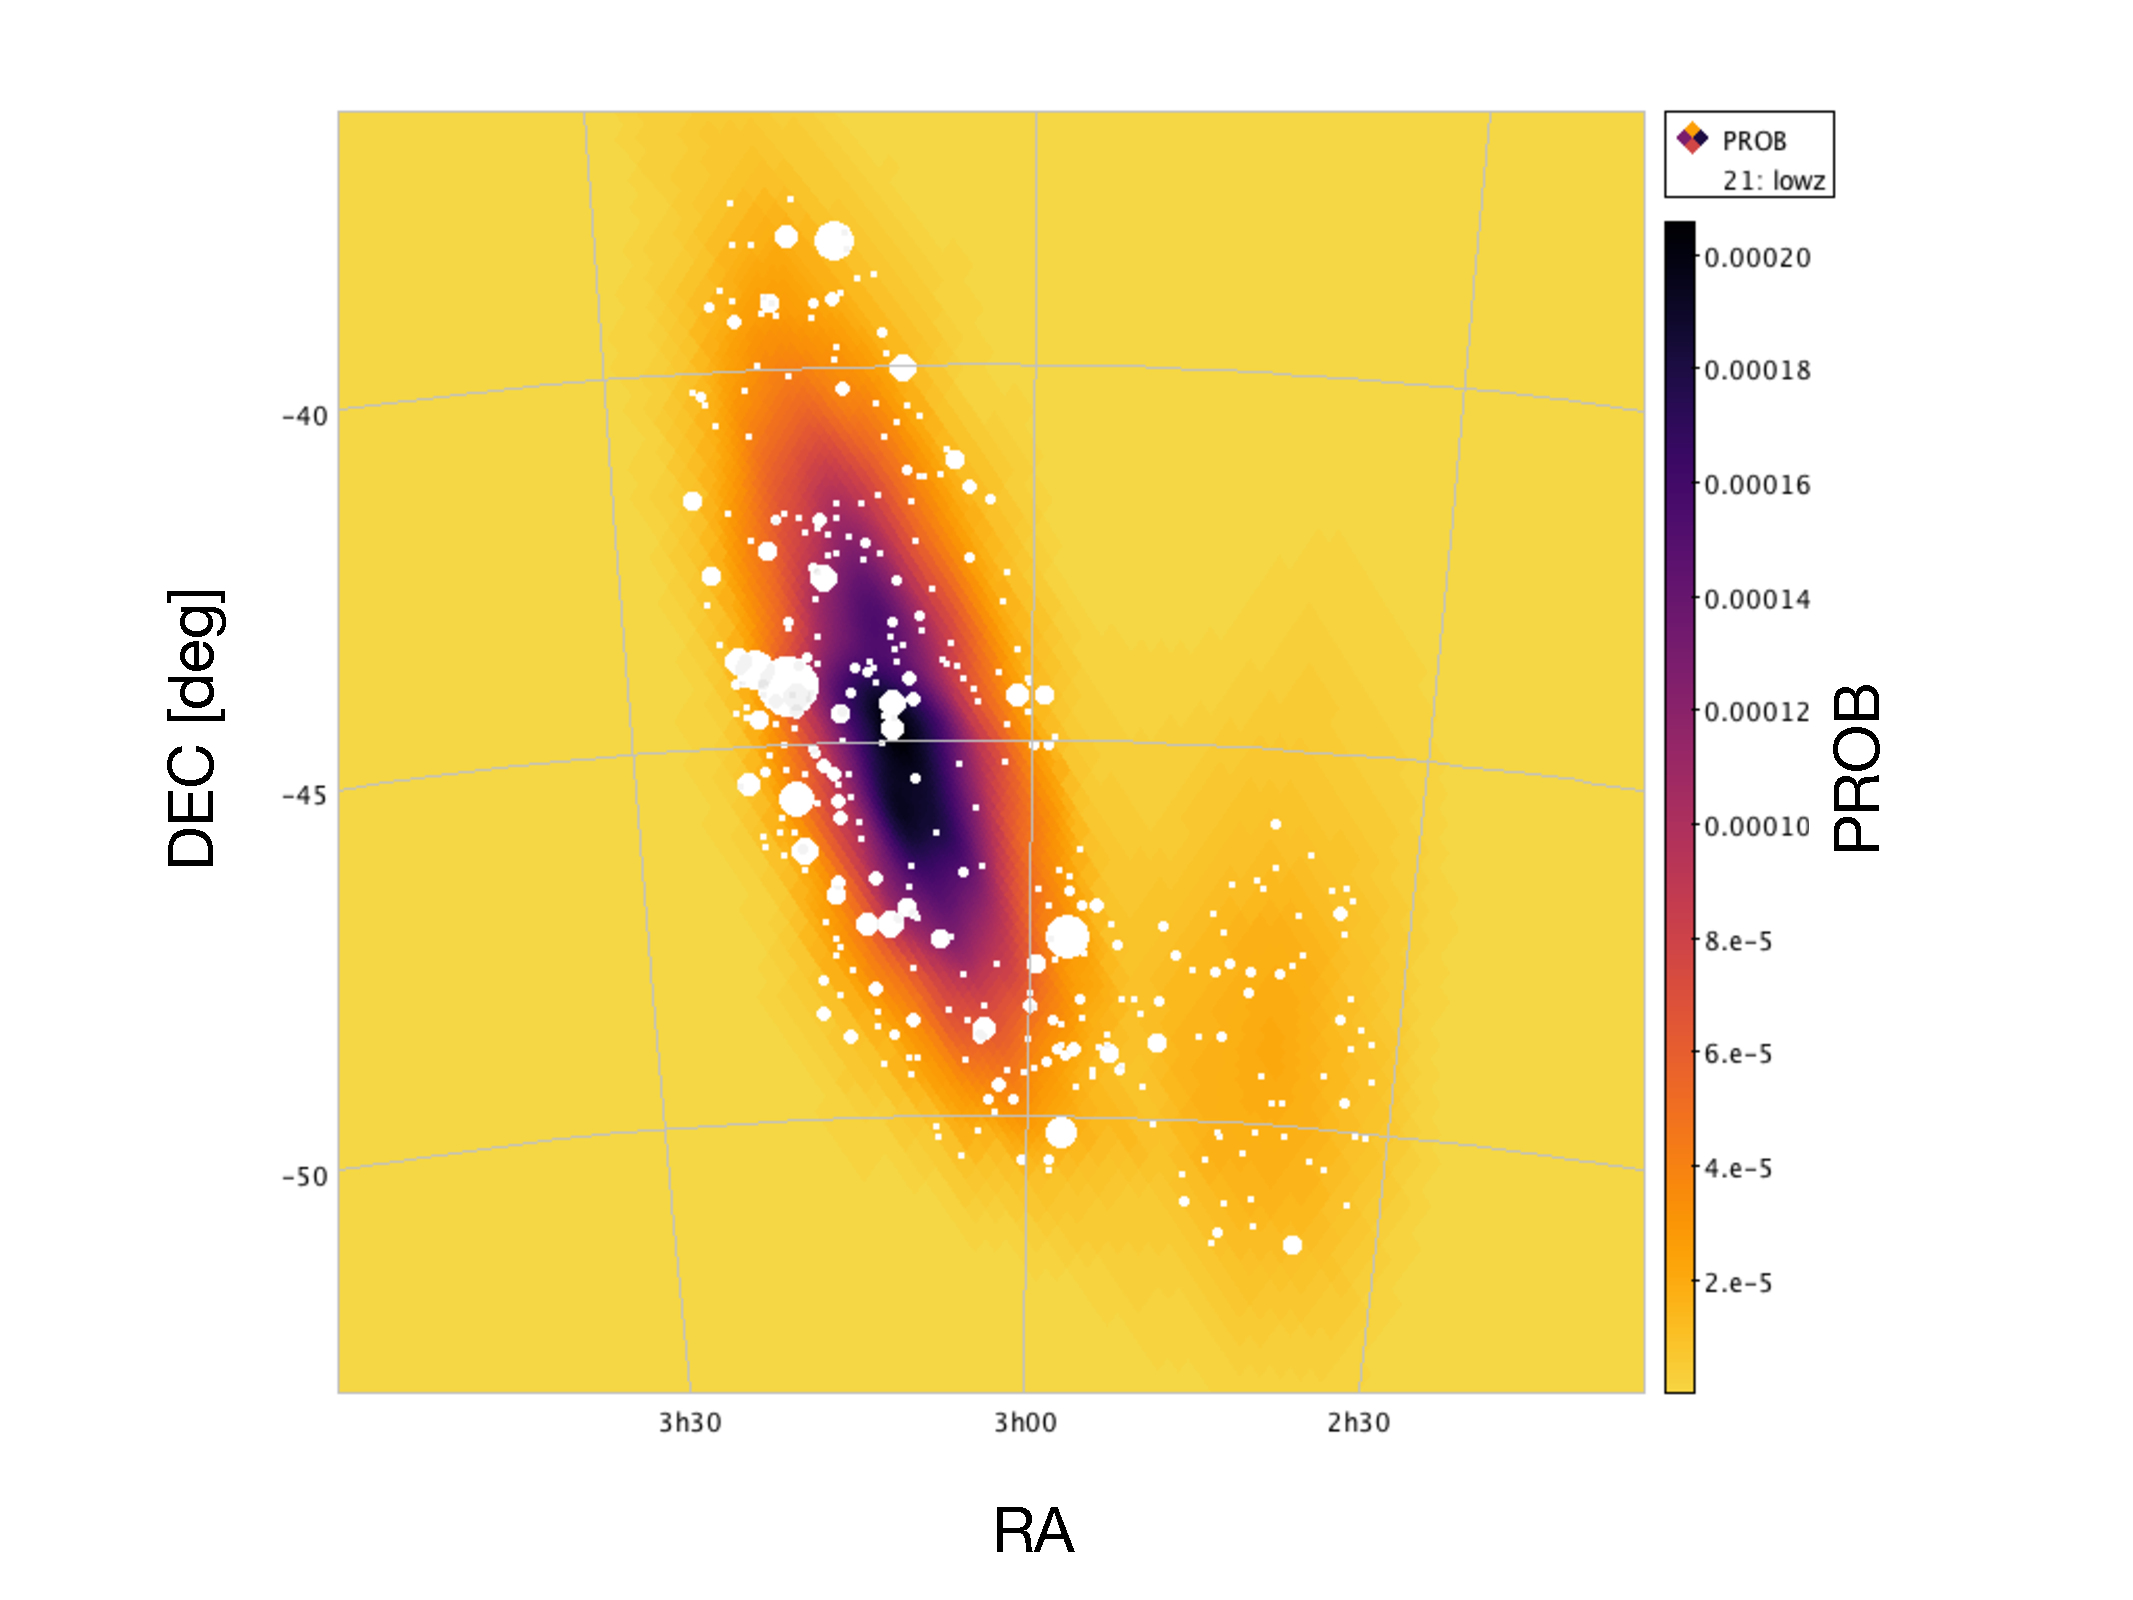
\includegraphics[width=0.75\textwidth]{./chapters/chapter8/GW170814.pdf}
\caption{The probability map from LIGO (density plot), and the Y3 redMaPPer groups and clusters at $z_{ph}<0.25$ within the 90\% probability area (white circles, where the radius is proportional to their richness).}\label{fig:GW170814}\end{figure}

The next LIGO observing season (O3; October 2018 -- September 2019), is expected to bring a 10--fold increase in number of detections: $\sim 8$ BNS events and $\sim 100$ BBH signals (computed from \citealt{2017arXiv170908079C}). I am involved in DECam and Gemini proposals to follow up LIGO O3 events, and obtaining photometry and spectra of the transients and host galaxies is part of the plan. If we are successful, I plan on extending the work presented here to future BNS events. If BBH events do no show any counterparts, the same analysis can still be carried out in a statistical way. I plan on implementing an observational methodology for cross-correlating galaxy catalogs with BBH GW events, given probability sky maps for each event. My method would incorporate full photometric redshift PDF information and a flexible prior on host galaxy properties. The host galaxy dependance will reveal information on BBH formation and nature (as suggested in e.g. \citealt{raccanelli}). From such analysis, there is also room for measurements of the Hubble constant: the GW event provides a distance measurement, and our galaxy catalogs will have computed photometric or spectroscopic redshifts. Measurements in this direction are extremely valuable means towards understanding the existing tensions between $H_0$ estimates from SNe and CMB experiments.

\section{Clusters}

\subsection{Conclusions from this thesis}
Stellar mass is regarded the most robust galaxy property that can be estimated from SED fitting. However, the typical uncertainty on photo-$z$'s can pose significant challenges for deriving this property if the galaxies' redshifts need to be assumed. Recent cluster finders, such as redMaPPer, are able to provide much excellent photo-$z$ estimates, so that this problem can be overcome. In Chapter \ref{chp:rxj}, I have presented an analysis on stellar mass estimation with early DES data for the galaxy cluster RXC J2248.7--4431. The opportunity for a consistency test is provided by the overlap with HST data, and we find that DES is able to estimate stellar masses within 25\% of HST values when the cluster redshift is assumed. Using the weak lensing measurements from \citet{melchior}, I have studied total stellar mass and stellar mass fraction profiles of this cluster out to the very large radii that DES is able to probe, thanks to the DECam wide field of view. Within $r_{200c}$ the stellar mass fraction is $\sim 0.7\%$, which is compatible with other results from the literature. This means that in this cluster only $\sim 4\%$ of the baryons are locked into stars. In the future, I plan on providing an estimate of the density in stars $\Omega_\star$ from the stellar masses I have computed from DES galaxies.

I have presented the follow up of the work on the stellar mass fraction in clusters in Chapter \ref{chp:chp6}. Using $\sim 76,000$ clusters from the DES Y1 redMaPPer sample, I show that $f_\star\sim 7\%$ and that the stellar mass fraction is roughly constant over the mass range $13.5<{\rm Log} (M_{200c})<14.5$. This indicates that the suppression of star formation efficiency at larger halo masses is not as strong as previously thought, and it is the contribution of satellites that makes this efficiency only a mild function of halo mass. The total cluster mass estimates are derived from weak lensing studies performed by DES collaborators.

I have also presented measurements of the stellar--to--halo mass relation for central galaxies, satellites and total cluster content for the same Y1 cluster sample. For the total content of clusters: $M_\star^{\rm tot}\propto M_{200c}^{0.89}$ with an intrinsic scatter at fixed halo mass of $0.2492\pm 0.0010$ ($1\sigma$ uncertainty). Central galaxies show a shallower slope (in logarithmic scale) in their relation with total mass ($\sim 0.4$). It is the satellites that contribute to the steepening of the total SHMR, as most of the stellar content resides there for increasing halo mass. The results presented are mostly in agreement with previous works, but they have been measured on a sample which is 1--3 orders of magnitude larger than other literature results. 

Chapter \ref{chp:chp6} also includes measurements of the stellar mass function in clusters. I have fit this with a log--normal distribution for the centrals, and a Schechter function for the overall galaxy population. The measured low mass end slope is $\alpha=-1.119\pm 0.025$ ($1\sigma$ uncertainty), with evidence of evolution over $0.1<z<0.7$. The high mass end shows no signs of evolution, implying that the mass build up of massive galaxies has ended by $z\sim 0.7$, as opposed to low mass galaxies that continue to evolve. I have contributed to the work on ICL detection lead by DES collaborator Yuanyuan Zhang. In particular, I have focused on colour and stellar mass measurements of this component. I have shown that the ICL becomes bluer toward larger cluster radii and that this is a consequence of different contributions to the diffuse light. In the core of the cluster, the central galaxy blends into the ICL, while towards larger radii dwarf disruption and tidal stripping are the most likely formation mechanisms of ICL. Moreover, ICL is an important component for cluster mass estimation: it can contribute up to $\sim 40\%$ of the total stellar mass within 100 kpc. I have also explored the effect of the assumed IMF on the results reported, which can be substantial: it can bias cluster stellar mass by up to $\sim0.27$ dex.

Estimating the total mass for DES clusters is necessary for cluster cosmology. The tight correlation found in the SHMR shows that cluster stellar mass is a good proxy for total mass. Chapter 5 has shown that our stellar mass based proxy $\mu_\star $ is a promising mass observable. By comparing it with X--ray temperatures, I have found that the scatter at fixed $\mu_\star$ is $\sigma_{{\rm Log}T_X|\mu_\star }\sim 0.15$ and $\sim 0.14$ for the \emph{XMM} and \emph{Chandra} samples respectively. I found that these values are competitive compared to results from the widely used redMaPPer richness. This mass proxy has also been calibrated with weak lensing analyses from SDSS data in work lead by DES collaborator Maria Pereira. 

\subsection{Future work}
Our $\mu_\star$ team is currently implementing the methodology developed in this thesis and in external work into the Voronoi--Tessellation cluster finder, and we will provide VT DES cluster catalogs with $\mu_\star$ measurements in the near future. This catalog will represent an interesting alternative to redMaPPer clusters: we have seen that the intrinsic width of the red sequence increases with redshift, so that red sequence--based cluster finders may face more difficulties in identifying clusters at higher $z$. Moreover, we will be able to provide measurements for both red sequence and blue cloud galaxies.

In this golden era of large astronomical surveys, I am stunned by the overwhelming amount of new data that we have the opportunity to utilise for an incredibly wide range of astrophysical studies. While we pave our way towards a gravitational wave precision cosmology program to complement the classical cosmological probes, significant mysteries remain on the astrophysics of the systems studied, dark matter, dark energy and colliding black holes. I look forward, as a scientist or a spectator, to new exciting discoveries about the dark components of the Universe to be unveiled.




